In order to evaluate and validate the approach proposed in this paper, we have
conducted experiments on simulated and real-world data. Real-world data
has been acquired with a static nodding Laser Range-Finder (LRF) setup. Two
different lasers have been mounted, namely a SICK LMS-200 and an Hockuyo
UTM-30LX. We also tested our method on a pedestrian robot equipped with a
downward-facing SICK LMS-151 LRF that generates 3D point cloud while moving.

\subsection{Experimental Conditions and Quantitative Measures}

For the nodding lasers setup, we have recorded 33 3D point clouds with multiple
viewpoints from a standard street scene. For the pedestrian robot scenario, data
has been generated from a tour in a city center.

A quantitative evaluation of our algorithm can be carried out under various
interrelated perspectives: curb location in $x,y$, curb height in $z$,
number of planes, assignment of DEM cells to planes, plane parameters, or
computation time. Since we do not have a labeling of the curb position from
the dataset, we evaluate the predictive accuracy of a model trained
with one point cloud to the others in a similar fashion as~\cite{faria10fitting}.
To this end, we collect 19 point clouds from the same position and perform
cross-validation. Concretely, we iteratively estimate the parameter set
$\{\hat{\Theta},\mathbf{\hat{L}}\}$ using one point cloud and evaluate the
predictive error on the 18 remaining ones. The quantitative measure is the Root
Mean Square (RMS) error of prediction:

\begin{equation}
\label{eqn:rmspred}
RMSEP=\sqrt{\frac{1}{M}\sum_{i=1}^M(\hat{\mu}_{h_i}-\mathbf{\hat{w}}_k^\text{T}
\boldsymbol{\phi}(\mathbf{c}_i))^ 2)},
\end{equation}

where $M$ is the number of valid cells in the point cloud being predicted and
$\mathbf{\hat{w}}_k$ corresponds to the trained component at the MAP state of
the CRF at $\mathbf{c}_i$.

In order to further analyze our model, we have sampled point clouds from known
mixture of linear regression parameters and also evaluated in this case the RMS
error of the predicted parameters $\hat{\Theta}$ against their ground truth. In
the case of synthetic data, predicted curb location and height, and assignment
of cells to planes, can also be quantitatively evaluated. Furthermore, we can
judge the robustness and validity of our algorithm on various situations such
as T-junctions or inclined planes.

\subsection{Qualitative Evaluation}
Before we proceed with the actual quantitative analysis, we want to give a
glimpse on some qualitative results that demonstrate the pertinence of our
approach.

In Fig.~\ref{fig:europa}, our pedestrian robot navigates in a city center and
label curbs while driving. Since the point cloud is reconstructed while the
robot drives, curbs can only be detected behind the robot in this specific
situation. DEM patches are labeled sequentially and we achieve on-line and
real-time performance.

\begin{figure}[t]
\centering
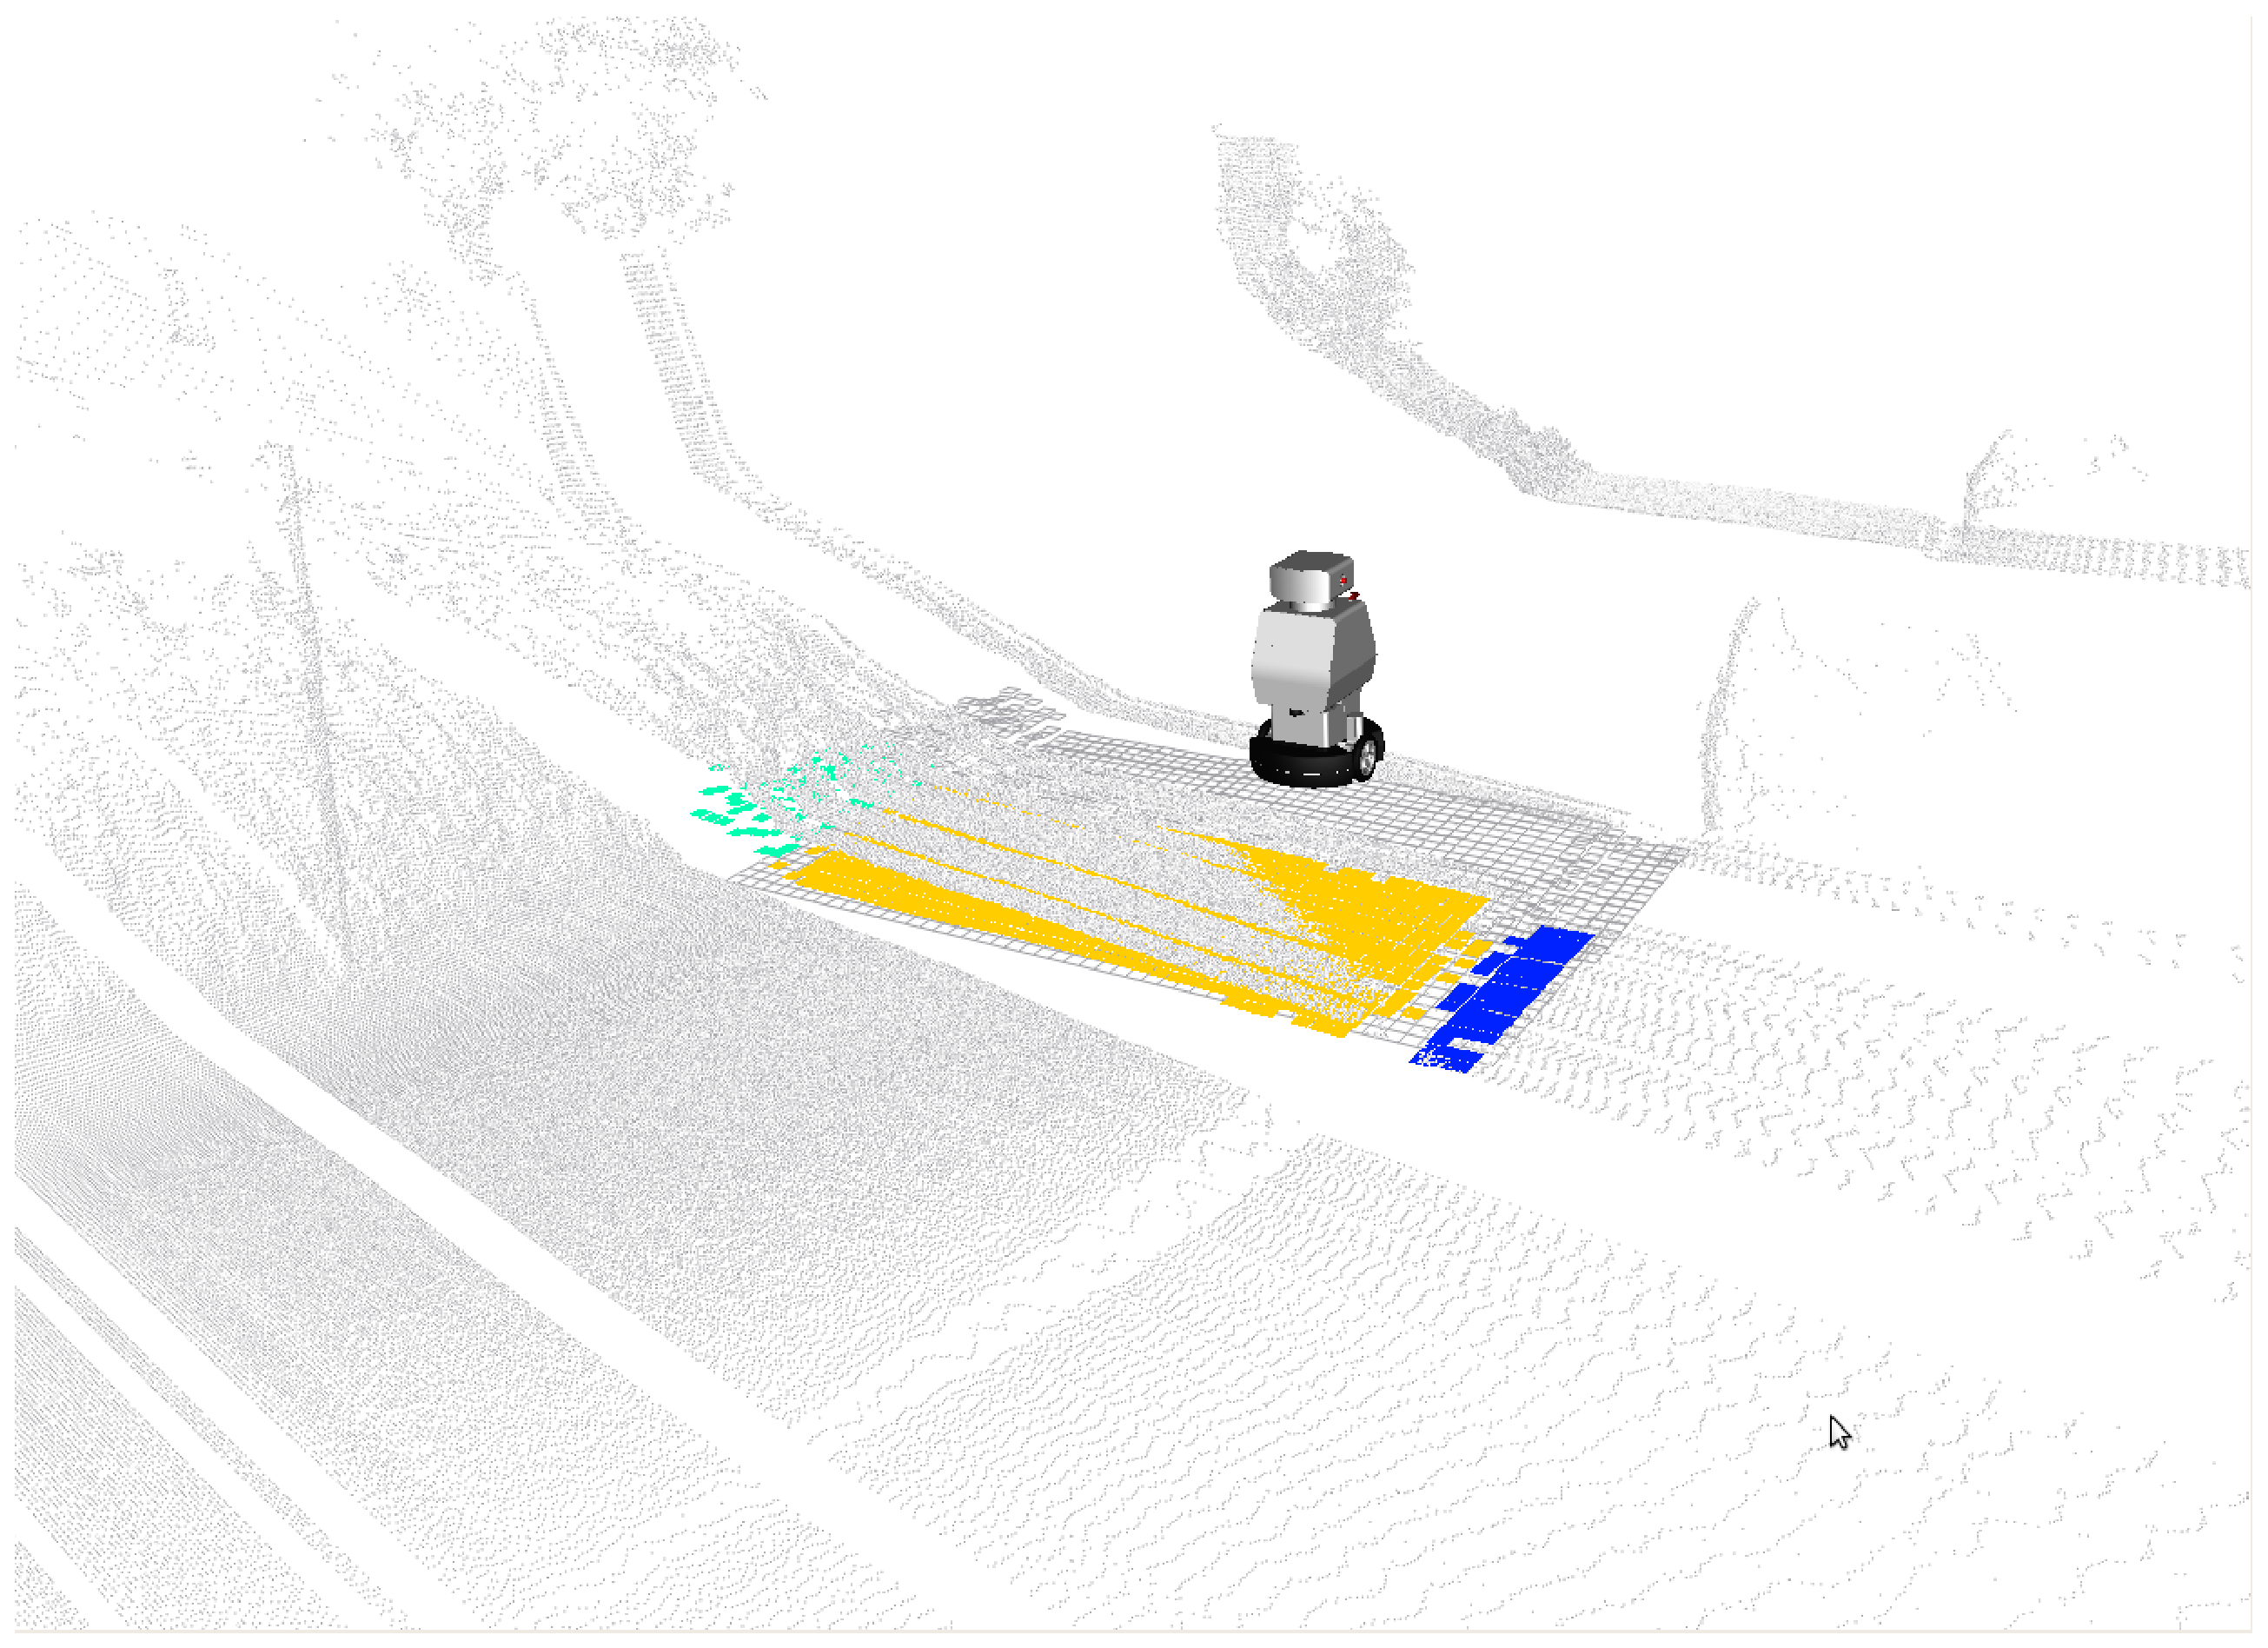
\includegraphics[width=\columnwidth]{fig/europa.eps}
\caption{Example of curb detection from a moving pedestrian robot. Colors
represent planes and curbs are located at their boundaries.}
\label{fig:europa}
\end{figure}

Fig.~\ref{fig:special} depicts a situation that a pedestrian robot might often
encounter when crossing a street. This experiment illustrates that our method
can cope with multiple viewpoints and environment configurations. Most of the
competitive approach would fail in this case.

\begin{figure}[t]
\centering
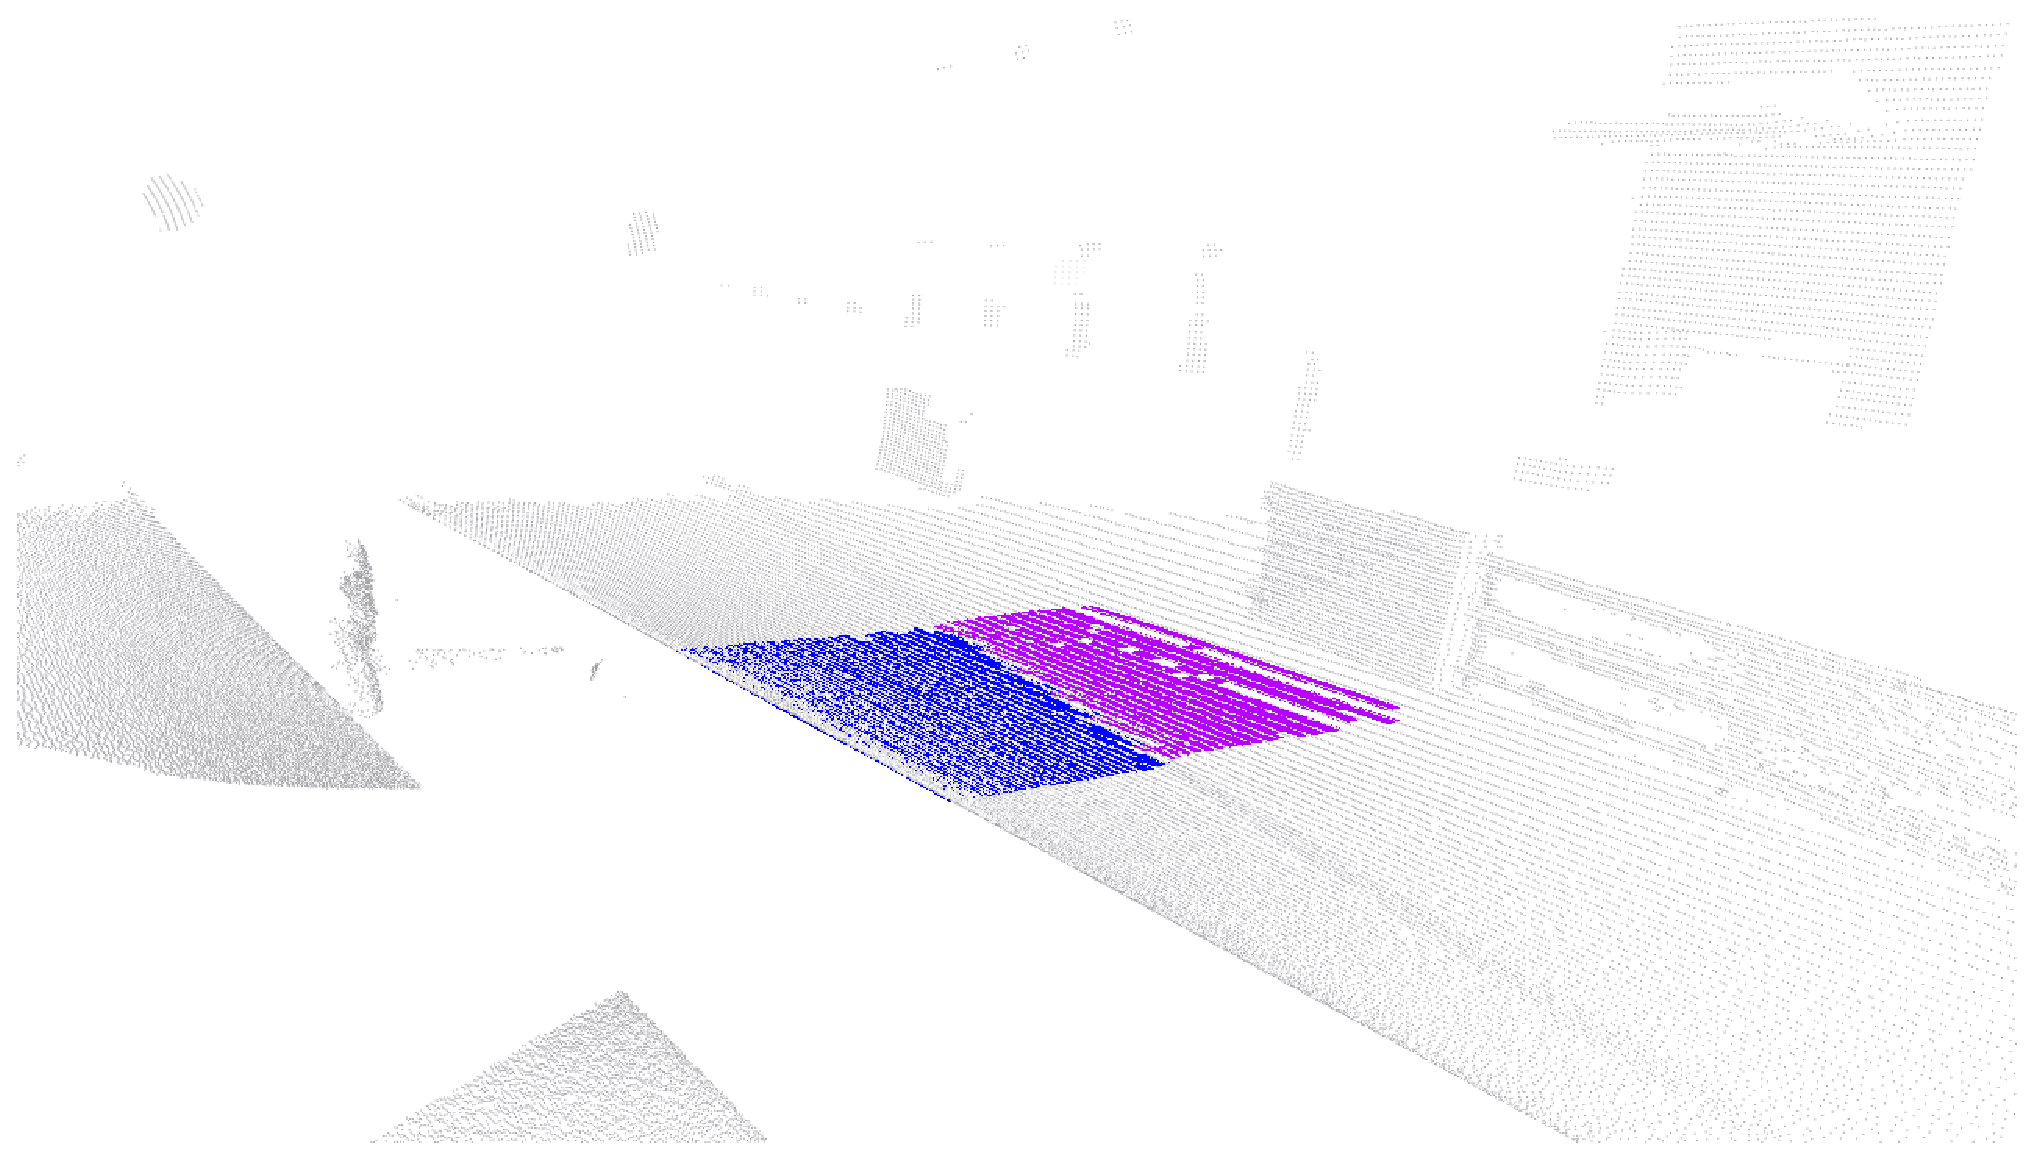
\includegraphics[width=\columnwidth]{fig/special.eps}
\caption{Example of curb detection in an unfavorable situation. Our algorithm
correctly label the planes, and thus curbs, under various viewpoints and
experimental settings.}
\label{fig:special}
\end{figure}

Fig.~\ref{fig:segment} displays the outcome of the segmentation algorithm on a
point cloud, while Fig.~\ref{fig:ml} shows the results obtained from the
standard EM algorithm. As a comparison, our method is applied on the same data
and the result is depicted on Fig.~\ref{fig:crf-em}. These experiments clearly
highlight the advantages of our method.

\begin{figure}[t]
\centering
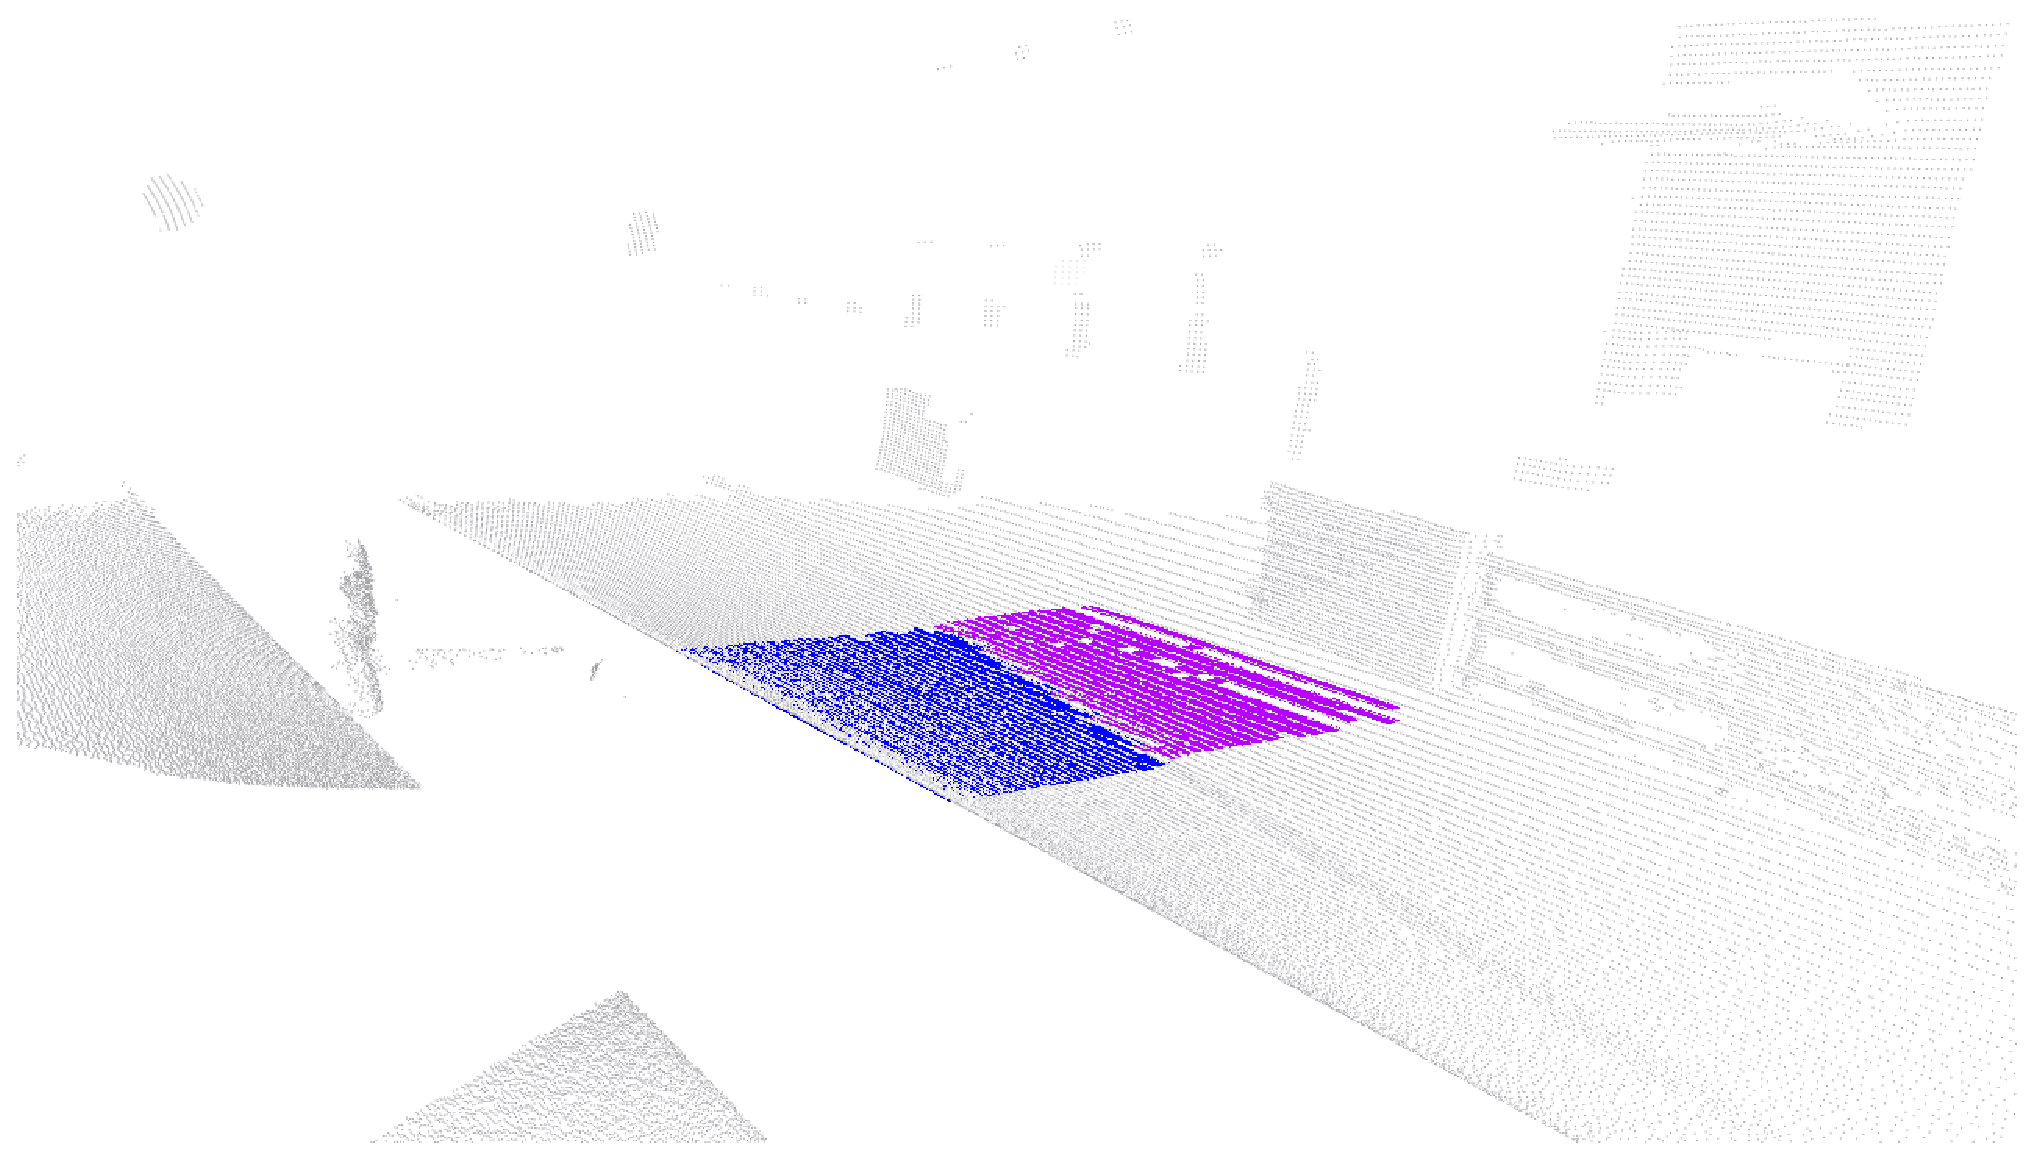
\includegraphics[width=\columnwidth]{fig/special.eps}
\caption{Example of curb detection in an unfavorable situation. Our algorithm
correctly label the planes, and thus curbs, under various viewpoints and
experimental settings.}
\label{fig:segment}
\end{figure}

\begin{figure}[t]
\centering
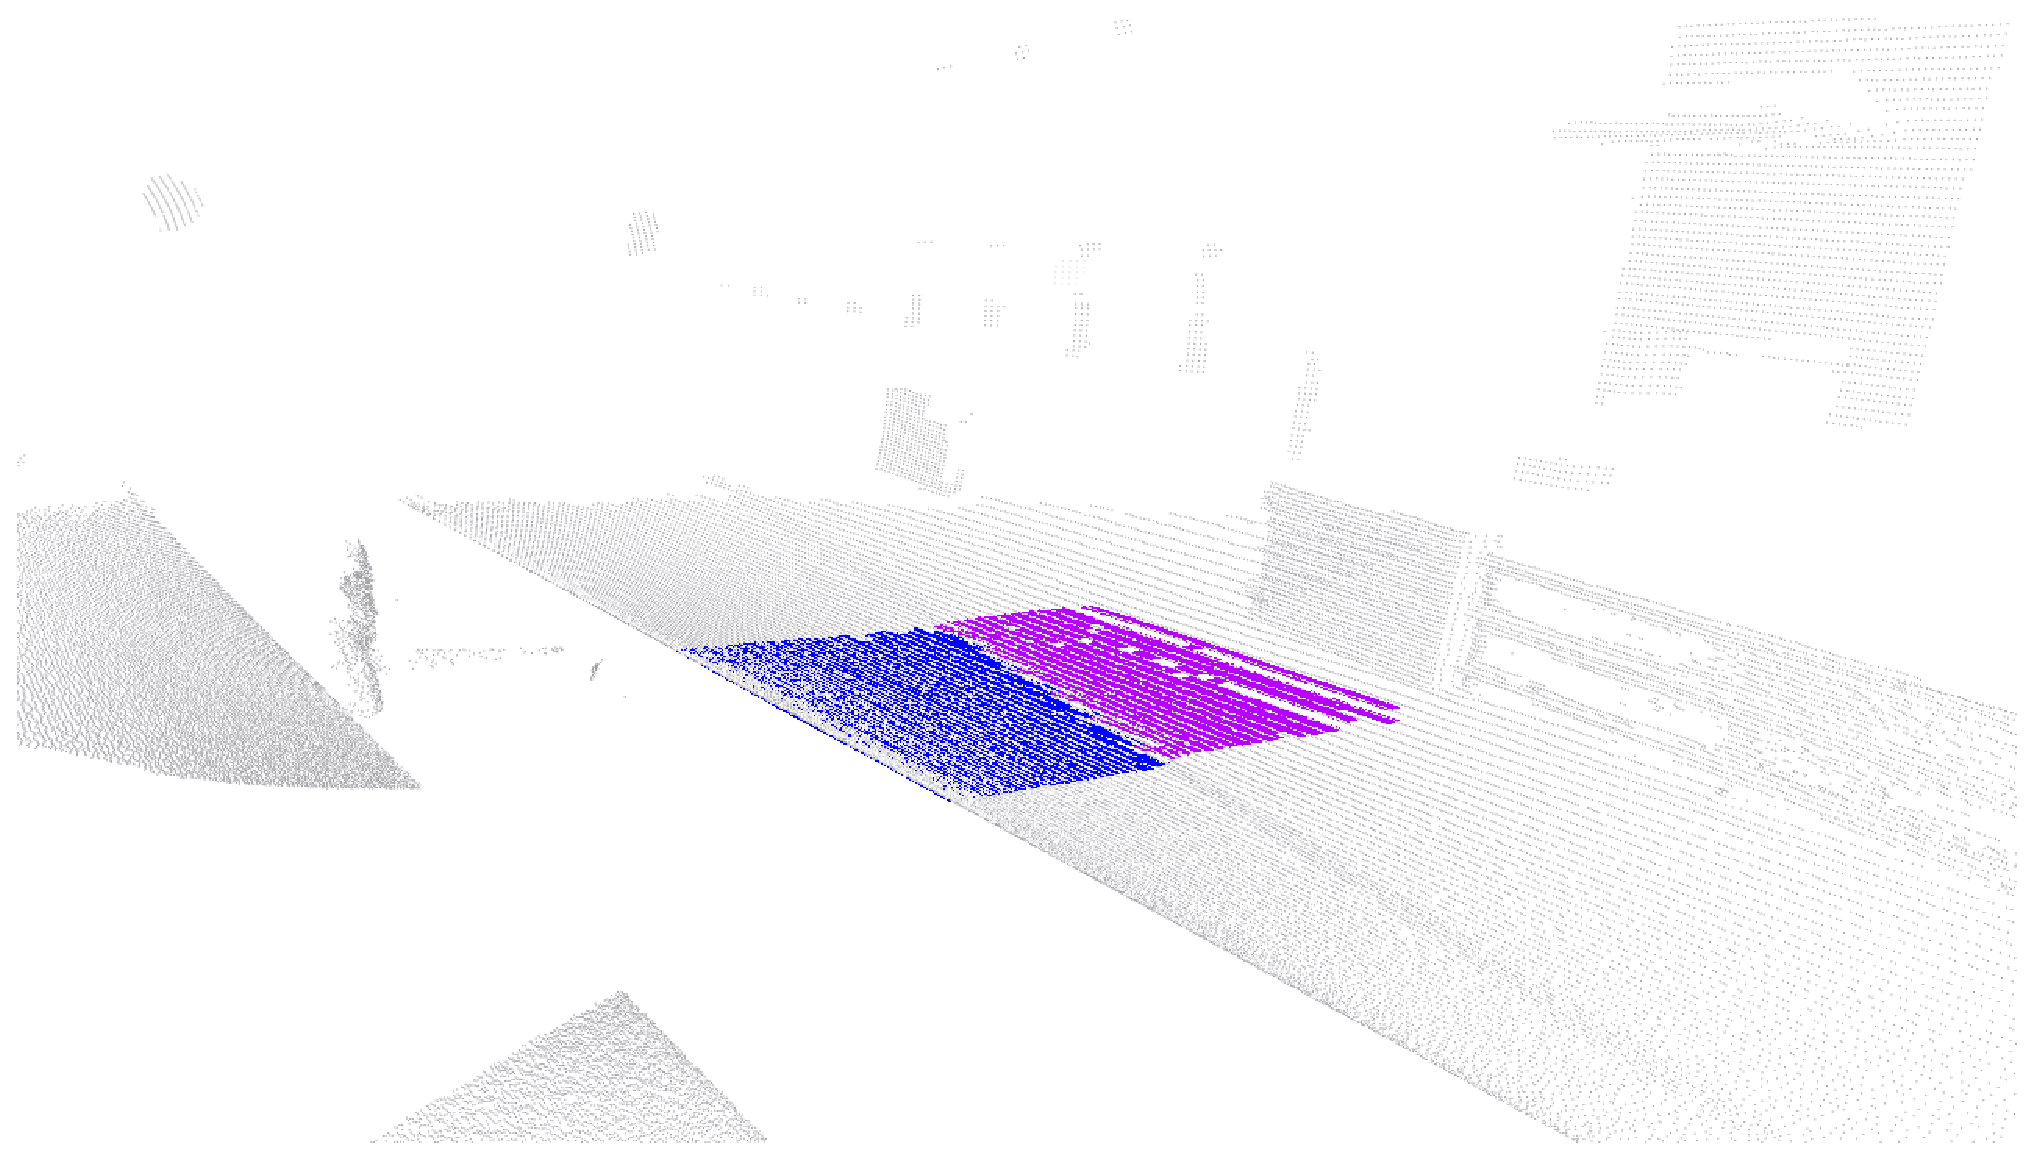
\includegraphics[width=\columnwidth]{fig/special.eps}
\caption{Example of curb detection in an unfavorable situation. Our algorithm
correctly label the planes, and thus curbs, under various viewpoints and
experimental settings.}
\label{fig:ml}
\end{figure}

\begin{figure}[t]
\centering
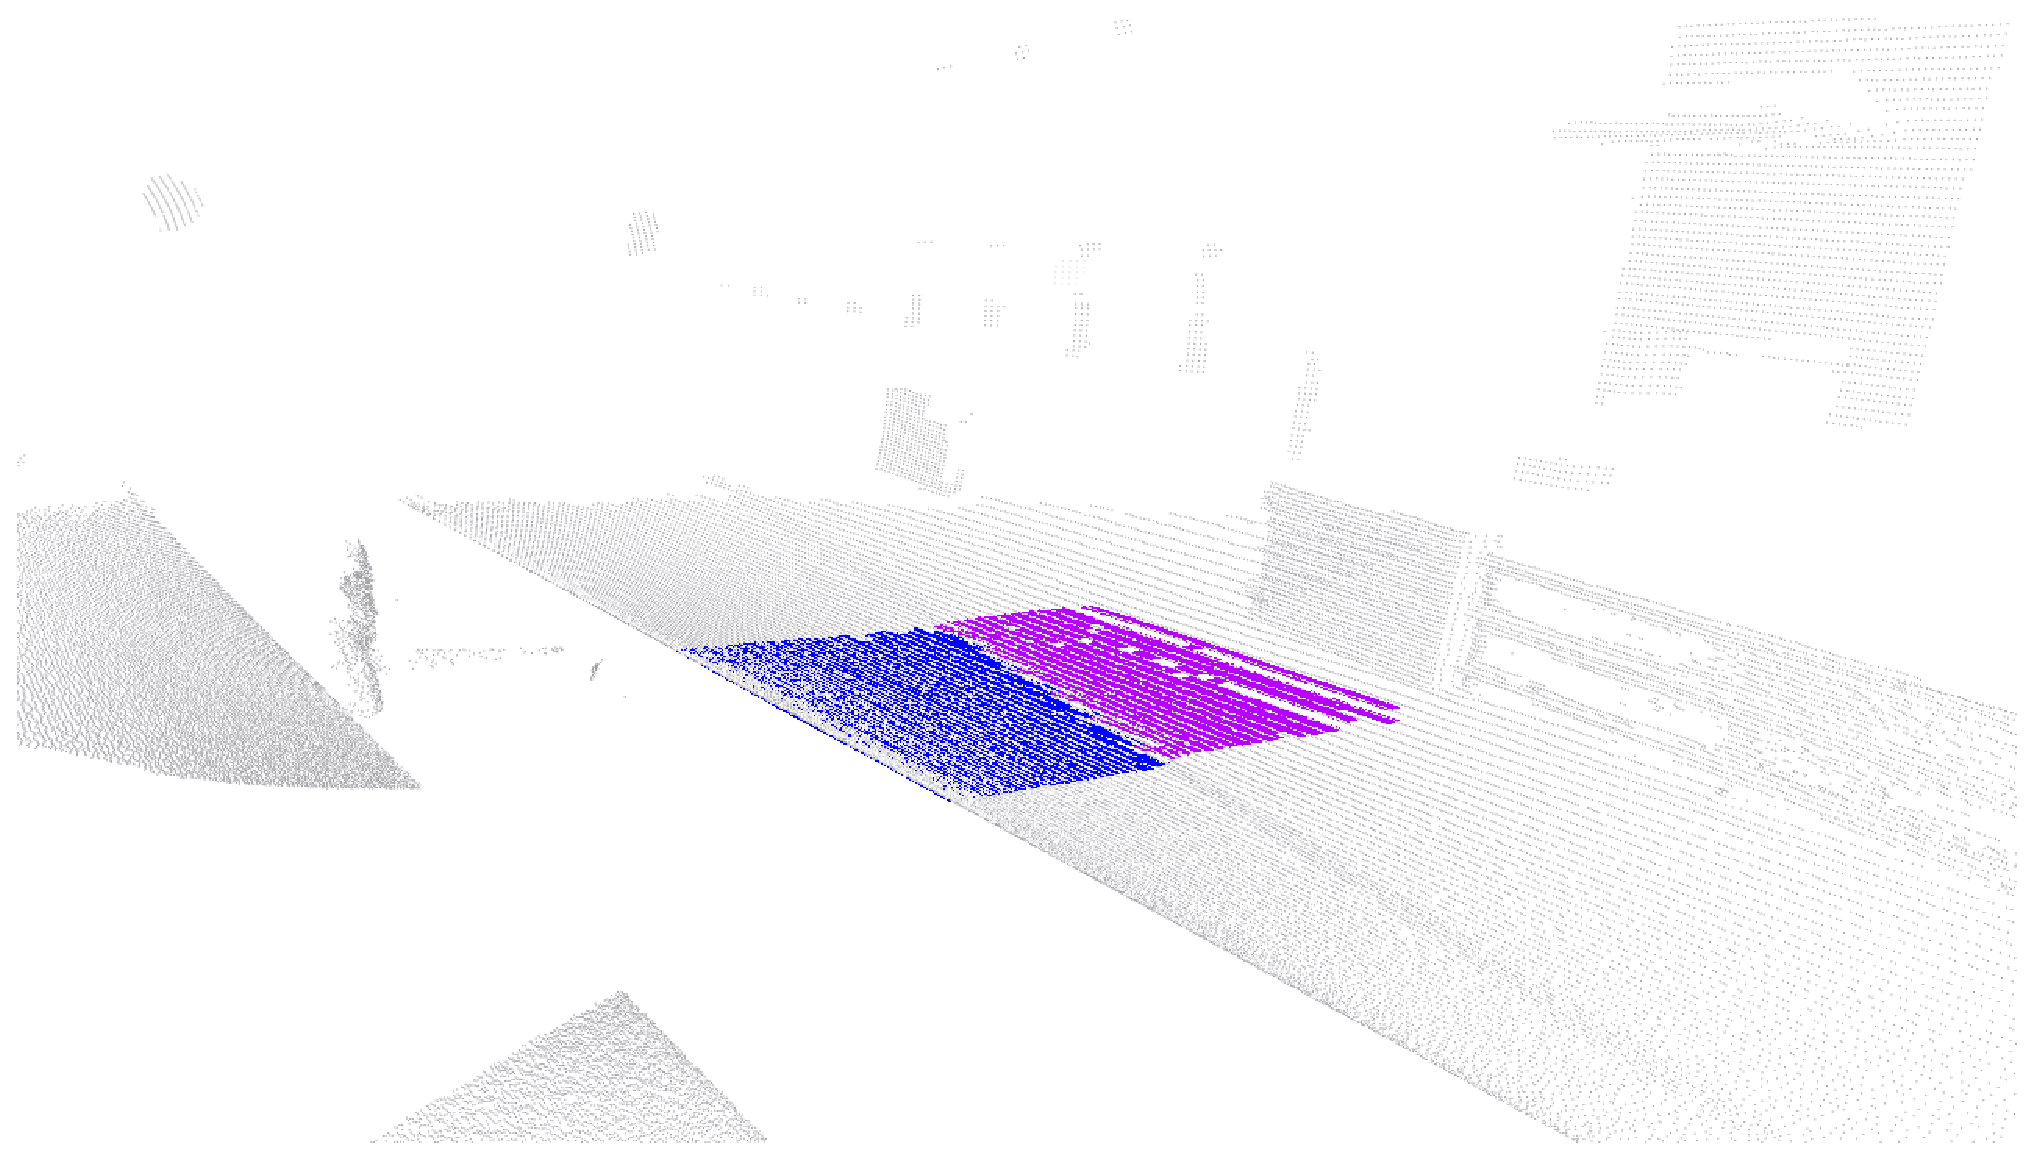
\includegraphics[width=\columnwidth]{fig/special.eps}
\caption{Example of curb detection in an unfavorable situation. Our algorithm
correctly label the planes, and thus curbs, under various viewpoints and
experimental settings.}
\label{fig:crf-em}
\end{figure}

\subsection{Quantitative Evaluation and Discussion}

\subsubsection{Real-World Data}

In order to further analyze our model, we have sampled point clouds from known
mixture of linear regression parameters and also evaluated in this case the RMS
error of the predicted parameters $\hat{\Theta}$ against their ground truth. In
the case of synthetic data, predicted curb location and height, and assignment
of cells to planes, can also be quantitatively evaluated. Furthermore, we can
judge the robustness and validity of our algorithm on various situations such
as T-junctions or inclined planes.

\subsubsection{Synthetic Data}

In order to further analyze our model, we have sampled point clouds from known
mixture of linear regression parameters and also evaluated in this case the RMS
error of the predicted parameters $\hat{\Theta}$ against their ground truth. In
the case of synthetic data, predicted curb location and height, and assignment
of cells to planes, can also be quantitatively evaluated. Furthermore, we can
judge the robustness and validity of our algorithm on various situations such
as T-junctions or inclined planes.
